\documentclass[handout]{beamer}
\mode<presentation> {%
	\usetheme[]{Boadilla}
	\usecolortheme{orchid}
	\setbeamercovered{transparent}
	\setbeamersize{text margin left=0.7cm}
  \setbeamersize{text margin right=0.7cm}
  \setbeamertemplate{enumerate item}[square]
  \setbeamertemplate{enumerate subitem}[circle]
  \setbeamertemplate{enumerate subsubitem}[>]
  \setbeamertemplate{itemize item}[square]
  \setbeamertemplate{itemize subitem}[circle]
  \setbeamertemplate{itemize subsubitem}[>]
}


\usepackage{bm}
\usepackage[utf8]{inputenc}
\usepackage[spanish]{babel}
\usepackage{times}
\usepackage[T1]{fontenc}
\usepackage{graphicx}
\usepackage{multirow}
\usepackage{pifont}
\usepackage{rotating}
\usepackage{colortbl}
\usepackage[framed]{mcode}
\usepackage{verbatim}
\usepackage{mathtools}
% \usepackage{tikz}
% \usetikzlibrary{positioning}
% \usetikzlibrary{shapes.multipart,decorations.pathreplacing}
% \tikzstyle{bloque}=[rectangle,rounded corners=2pt,draw=black!60,fill=black!5,very thick,minimum size=5mm,align=center]%
% \tikzstyle{arrow}=[very thick,color=black!60]%


\definecolor{olivegreen}{rgb}{0.0,0.5,0.0}
% \definecolor{general}{rgb}{0.9 0.9 1}%
% \newrgbcolor{colorsistema}{0 1 1}
% \newrgbcolor{colorviolet}{0.9 0.8 1}

\author[J. Chacón]{%[Author, Another] % (optional, use only with lots of authors)
\textit{Ingeniería Electrónica de Comunicaciones }\\
\vspace{0.6cm}
\small Jesús Chacón Sombría}%\inst{1} \and S.~Another\inst{2}}


\institute[DACYA. UCM] % (optional, but mostly needed)
{
  %\inst{1}%

\footnotesize  Departamento de Arquitectura de Computadores y Automática.\\
  Universidad Complutense de Madrid
  }

\date[Diseño de filtros] % (optional)
{\footnotesize Curso 2025-2026}%{\today / Master}
\subject{Talks}

\pgfdeclareimage[height=0.75cm]{logo}{ucm}

\usepackage[absolute,overlay]{textpos}
\setlength{\TPHorizModule}{1mm}
\setlength{\TPVertModule}{1mm}
\newcommand{\MyLogo}{%
\begin{textblock}{14}(116.0,0.6)
  \pgfuseimage{logo}
\end{textblock}
}

\makeatletter
\numberwithin{section}{part}
\AtBeginPart{
\beamer@tocsectionumber=0\relax
\frame{\partpage}
}
\makeatother

\begin{document}

\begin{frame}
  \titlepage
\end{frame}

\newcommand*\oldmacro{}%
\let\oldmacro\insertshorttitle%
\renewcommand*\insertshorttitle{%
 \MyLogo
  \oldmacro\hfill%
}

\AtBeginSection[]{}
\AtBeginSubsection[]{}

\subsection{Filtros FIR}

\begin{frame}
  \frametitle{Procedimiento de diseño de filtros FIR}
  
  \[
  y[n]=\substack{N-1\\\sum\\k=0}x[n-k]
  \]
  \[\color{blue}
  h[n]=\substack{N-1\\\sum\\k=0}b_k \delta[n-k]
  \Leftrightarrow
  H(\omega)=\substack{N-1\\\sum\\k=0}b_k \mathrm{e}^{-j\omega k}
  \]
  
  \alert{¿Cómo diseñamos filtros FIR?}
  \begin{itemize}
    \footnotesize
    \item No tienen conexión directa con ningún filtro continuo.
    \item Su diseño no se puede basar en la aproximación de un filtro analógico.
  
    % \item Aproximación directa de la respuesta en frecuencia (i.e. calcular los valores de $h(n)$ para que $H(e^{jw})$ tenga la forma deseada).
  
  % \hspace{0.8cm}$H(\omega})=\sum_{n=-\infty}^{\infty} h(n)e^{-jwn} \rightarrow H(e^{jw})=\sum_{n=0}^{N} h(n)e^{-jwn} $
  
    \item Los filtros que vamos a estudiar cumplen dos propiedades adicionales\footnote{Para que el desfase introducido a cada frecuencia sea $-\omega N/2$.}:
    \begin{itemize}
      \footnotesize
      \item \textbf{Coeficientes reales}: $h[n]=h^{*}[n]$.
      \item Respuesta de \textbf{fase lineal}: $arg(H(\omega))=\alpha\omega+\beta$. 
    \end{itemize}

    \item Métodos de diseño:
    \begin{itemize}
      \footnotesize
      \item Transformada de Fourier con ventana.
      \item \color{gray} Muestreo en frecuencia.\color{black}
      \item Diseño asistido por computador.
    \end{itemize}
    
  \end{itemize}
  
\end{frame}


\begin{frame}
  \frametitle{Diseño FIR por TF con ventana}
  
  \vspace{-0.2cm}
  \begin{itemize}
    \item La respuesta impulso de un filtro ideal es:
    \begin{itemize}
      \item de longitud infinita (IIR).
      \item no causal ($h_d[n]\neq0$ para $n<0$).
    \end{itemize}
    \item \alert{Para convertir en un FIR de orden $N+1$ realizable:}
    \begin{enumerate}
      \footnotesize
      \item Truncamos la respuesta al impulso (limitar a $N+1$ coeficientes),  
      \begin{center}$\color{blue}h_w[n]=w[n]h_d[n]$ con una ventana $w[n]$ de tamaño $N+1=2L+1$.\end{center}
      \item Retardamos $L=\frac{N}{2}$ muestras, para hacerlo causal: $\color{blue}h[n]=h_d[n-L]$. 
    \end{enumerate}
    \item El filtro FIR obtenido es de fase lineal, ya que:
    \begin{itemize}
      \item El filtro ideal es de fase cero: $arg~H_d(\omega)=0$.
      \item El truncamiento no modifica la fase.
      \item El retardo añade un desfase proporcional a la frecuencia:
      \begin{center}$\color{blue}H(\omega)=e^{-jL\omega}H_w(\omega)=e^{-j\omega\frac{N}{2}}H_w(\omega)$.\end{center}
    \end{itemize}
  \end{itemize}
  
\end{frame}


\begin{frame}
  \frametitle{Respuesta al impulso de filtros ideales}
  \footnotesize 
  \begin{itemize}
    \item Aplicando la transformada inversa de Fourier: \color{blue}$h_d[n]\!=\frac{1}{2\pi}\int_{-\pi}^\pi H_d(\omega) e^{j\omega n} d\omega$\color{black}.
  \end{itemize}
  
  \begin{columns}[T]
    \begin{column}{5cm}
    \scriptsize\centering
    \alert{Filtro paso bajo}

    \vspace{0.2cm}
    $H_{lp}(\omega)=\begin{cases}1~\mathrm{si}~|\omega|\leq\omega_c\\0~\mathrm{si}~|\omega|>\omega_c\end{cases}$

    \vspace{0.2cm}
    $h_{lp}[n]=\left\{\begin{matrix*}[l]
      \frac{\omega_c}{\pi} & \mathrm{si}~n=0\\\frac{\mathrm{sin}(\omega_c n)}{\pi n} & \mathrm{si}~n\neq 0
    \end{matrix*}\right.$

    \vspace{0.5cm}
    \alert{Filtro paso alto}

    \vspace{0.1cm}
    $H_{hp}(\omega)=\begin{cases}0~\mathrm{si}~|\omega|\leq\omega_c\\1~\mathrm{si}~|\omega|<\omega_c\end{cases}$

    \vspace{0.1cm}
    \color{gray}
    $H_{hp}(\omega)=1 - H_{lp}(\omega)$

    \vspace{0.1cm}
    $h_{hp}[n]=\delta[n] - h_{lp}[n]$
    \color{black}

    \vspace{0.1cm}
    $h_{hp}[n]=\left\{\begin{matrix*}[l]
      1-\frac{\omega_c}{\pi} & \mathrm{si}~n=0\\
      -\frac{\mathrm{sin}(\omega_c n)}{\pi n} & \mathrm{si}~n\neq 0
    \end{matrix*}\right.$
    
  \end{column}
    \begin{column}{5.5 cm}
    \scriptsize\centering
    \alert{Filtro paso banda}

    \vspace{0.1cm}
    $H_{bp}(\omega)=\begin{cases}1~\mathrm{si}~\omega_{c_1}\leq|\omega|\leq\omega_{c_2}\\0~\mathrm{c.c.}\end{cases}$

    \vspace{0.1cm}
    \color{gray}
    $H_{bp}(e^{j\omega})=H_{hp,\omega_{c_1}}(\omega)-H_{hp,\omega_{c_2}}(\omega)$
    \color{black}

    \vspace{0.1cm}
    $h_{bp}[n]=\left\{\begin{matrix*}[l]
      \frac{\omega_{c_2} - \omega_{c_1}}{\pi} & \mathrm{si}~n=0\\
      \frac{\mathrm{sin}(\omega_{c_2} n) - \mathrm{sin}(\omega_{c_1} n)}{\pi n} & \mathrm{si}~n\neq 0
    \end{matrix*}\right.$
    
    \vspace{0.1cm}    
    \alert{Filtro supresor banda}

    \vspace{0.1cm}
    $H_{bs}(\omega)=\begin{cases}0~\mathrm{si}~\omega_{c_1}\leq|\omega|\leq\omega_{c_2}\\1~\mathrm{c.c.}\end{cases}$

    \vspace{0.1cm}
    \color{gray}
    $H_{bs}(\omega)=1 - H_{bp}(\omega)$

    \vspace{0.1cm}
    $h_{bs}[n]=\delta[n] - h_{bp}[n]$
    \color{black}

    \vspace{0.1cm}
    $h_{bs}[n]=\left\{\begin{matrix*}[l]
      1 - \frac{\omega_{c_2} - \omega_{c_1}}{\pi} & \mathrm{si}~n=0\\
      -\frac{\mathrm{sin}(\omega_{c_2} n) - \mathrm{sin}(\omega_{c_1} n)}{\pi n} & \mathrm{si}~n\neq 0
    \end{matrix*}\right.$
    
    \end{column}
  \end{columns}
\end{frame}


\begin{frame}
  \frametitle{Respuesta al impulso de filtros ideales}
  \footnotesize
  
  \begin{itemize}
    \footnotesize
    \item De forma general, podemos definir un \textbf{filtro multibanda} ideal:
    \begin{itemize}
      \footnotesize
      \item $M$ bandas de amplitud $A_k$, para $k=1,...,M$.
      \item bordes de banda $\omega_k$, para $k=0,1,...,M~(\omega_0=0,\omega_M=\pi)$.
    \end{itemize}
  \end{itemize}
  \begin{columns}
    \begin{column}{0.38\textwidth}
      \vspace{0.5cm}
      \centering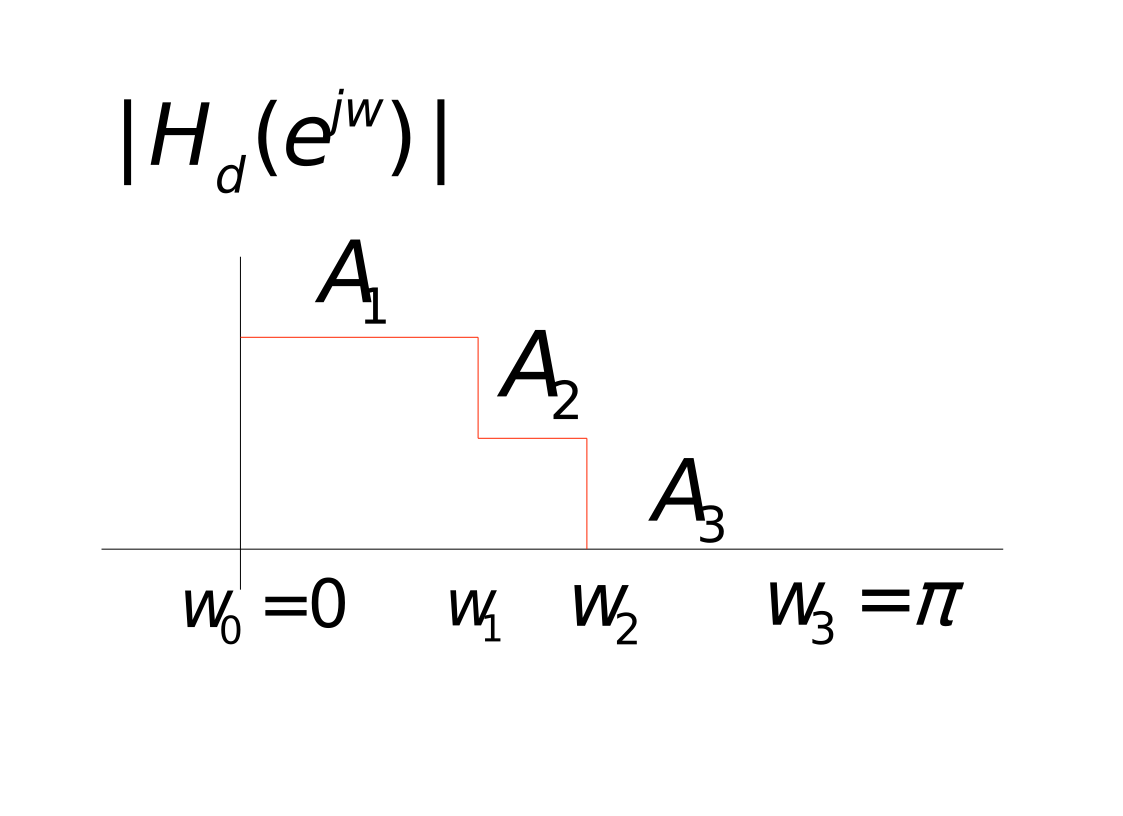
\includegraphics[trim=0cm 1cm 4cm 1cm,clip=true,width=3.5cm]{Figures/PorTramos}
    \end{column}
    \begin{column}{0.62\textwidth}
      \begin{flushleft}
      
      $H_{mb}(\omega)=A_k~\mathrm{si}~\omega_{k-1}\leq|\omega|\leq\omega_{k}, \mathrm{para}~k=1,...,M.$

      \vspace{0.4cm}
      \color{gray}$H_{mb}(\omega)=\substack{M\\\sum\\k=1}A_k H_{bp_{[\omega_{k-1},\omega_{k}]}}(\omega)$\color{black}

      \vspace{0.4cm}\color{blue}
      $h_{mb}[n]=\left\{\begin{matrix*}[l]
          \substack{M\\\sum\\k=1}A_k \frac{\omega_k - \omega_{k-1}}{\pi} & \mathrm{si}~n=0\\[2ex]
          \substack{M\\\sum\\k=1}(A_{k} - A_{k-1}) \frac{\mathrm{sin}(\omega_k n)}{\pi n} & \mathrm{si}~n\neq 0
        \end{matrix*}\right.$\color{black}
      \end{flushleft}
    \end{column}
  \end{columns}  
\end{frame}
  
%   \begin{frame}
%   \frametitle{Diseño del filtro FIR por truncamiento I}
  
%   \footnotesize
  
%   \begin{itemize}
%   \item EL filtro FIR correspondiente se puede diseñar truncando la función $h_d(n)$ correspondiente, haciéndola  cero para valores $|n|>L$ y retardándola L unidades temporales.
  
  
%   \visible<2->{
%   \item A continuación vemos la respuesta en frecuencia de los filtros así obtenidos para diferentes valores de N:
  
%   \vspace{-0.4cm}
  
  
  
%   \begin{columns}[c]
%   \begin{column}{5cm}
%   \lstinputlisting{./Matlab/FIRLowTrunc.m}
  
  
%    \end{column}
%   \hspace{-0.5cm} \begin{column}{5cm}
  
%   \centering
  
%   \visible<3->{
  
%   \scriptsize
%   Filtro paso bajo
  
  
  
%   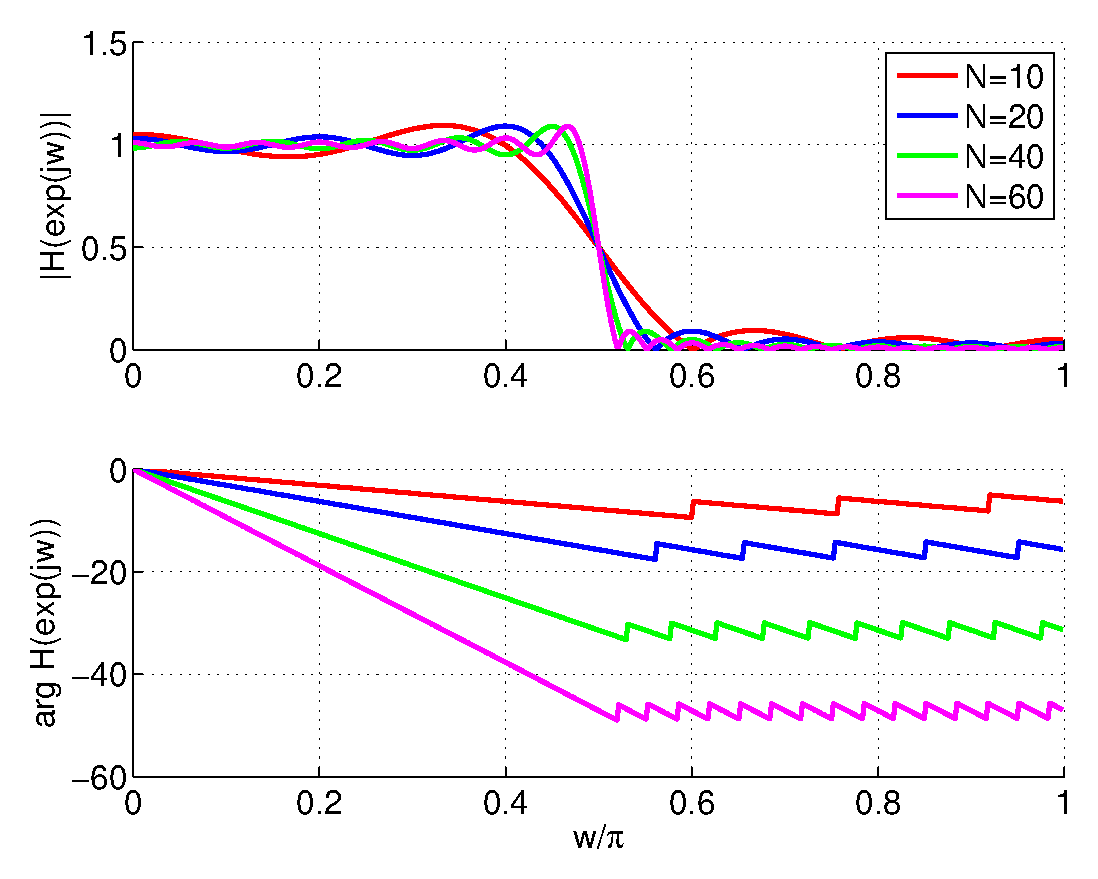
\includegraphics[width=5cm]{Figures/FIRLowTrunc.eps}
%   }
  
%   \visible<4->{
%   Desfase lineal ($-wN/2$, discont. $\pi$)
  
%   $N$ crece $\rightarrow \#_{rizos}$ crece
  
%   Tamaño rizos es constante.
%   }
%    \end{column}
%    \end{columns}
%   }
  
  
%   \end{itemize}
  
%   \end{frame}
  
%   %%%%%%%%%%%%%%%%%%%%%%%%%%
  
\begin{frame}
  \frametitle{Diseño del filtro FIR por truncamiento}
  
  \begin{columns}[c]
    \begin{column}{5cm}
      \centering
      \scriptsize
      
      Paso bajo
      
      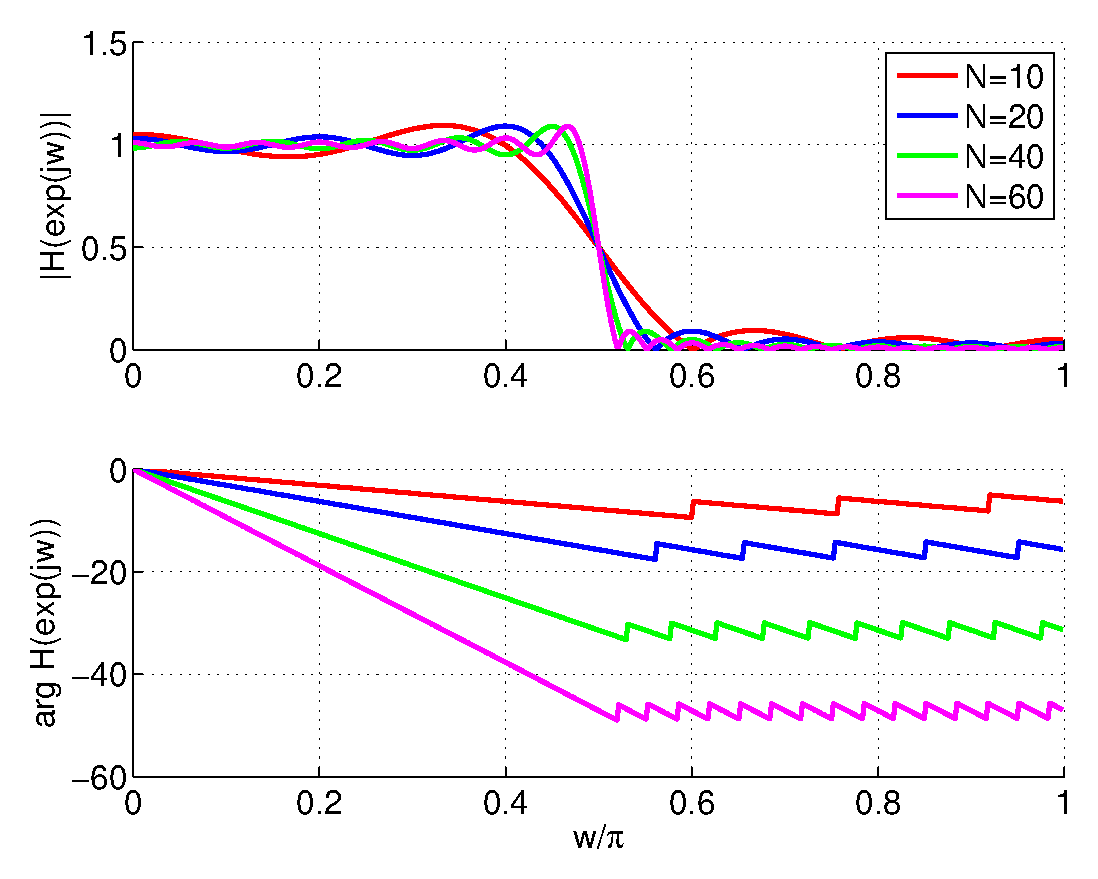
\includegraphics[width=4cm]{Figures/FIRLowTrunc.eps}
    
      Paso alto
      
      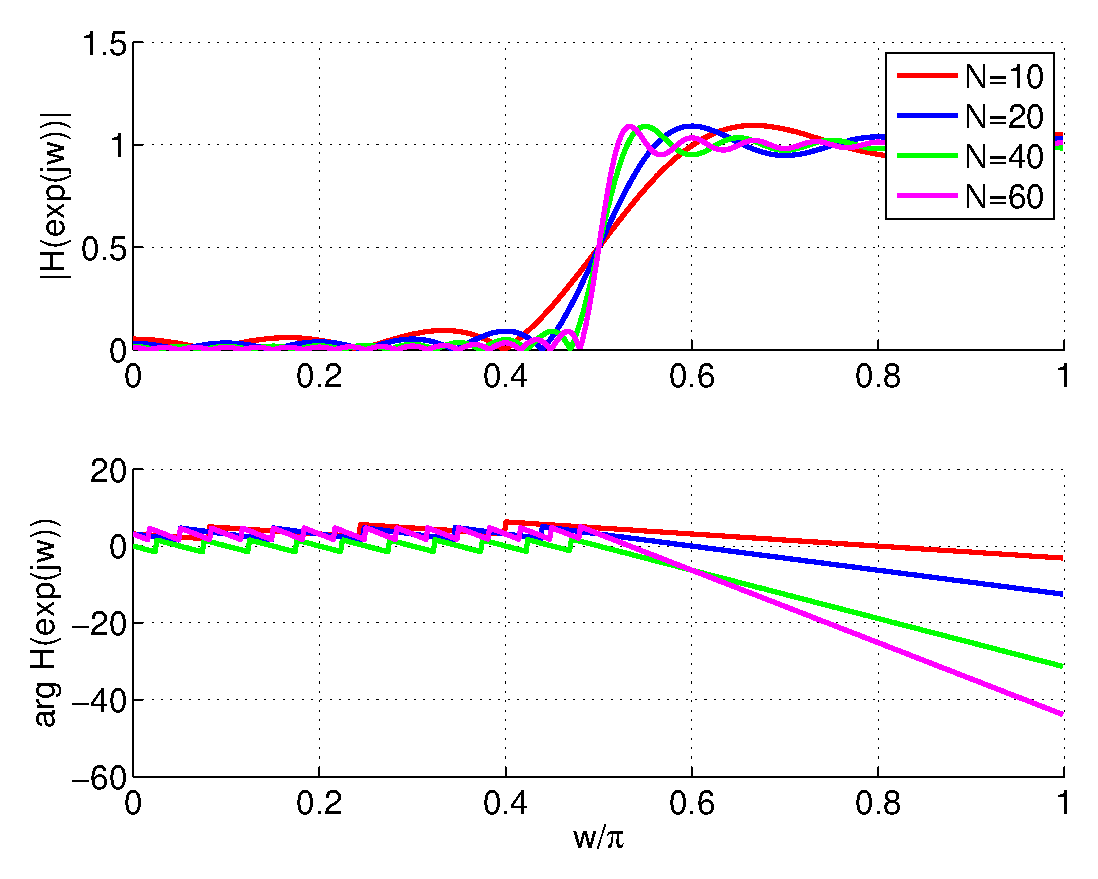
\includegraphics[width=4cm]{Figures/FIRHighTrunc.eps}   
    \end{column}
    \hspace{-0.5cm} \begin{column}{5cm}
      \scriptsize      
      Paso banda
      \centering
      
      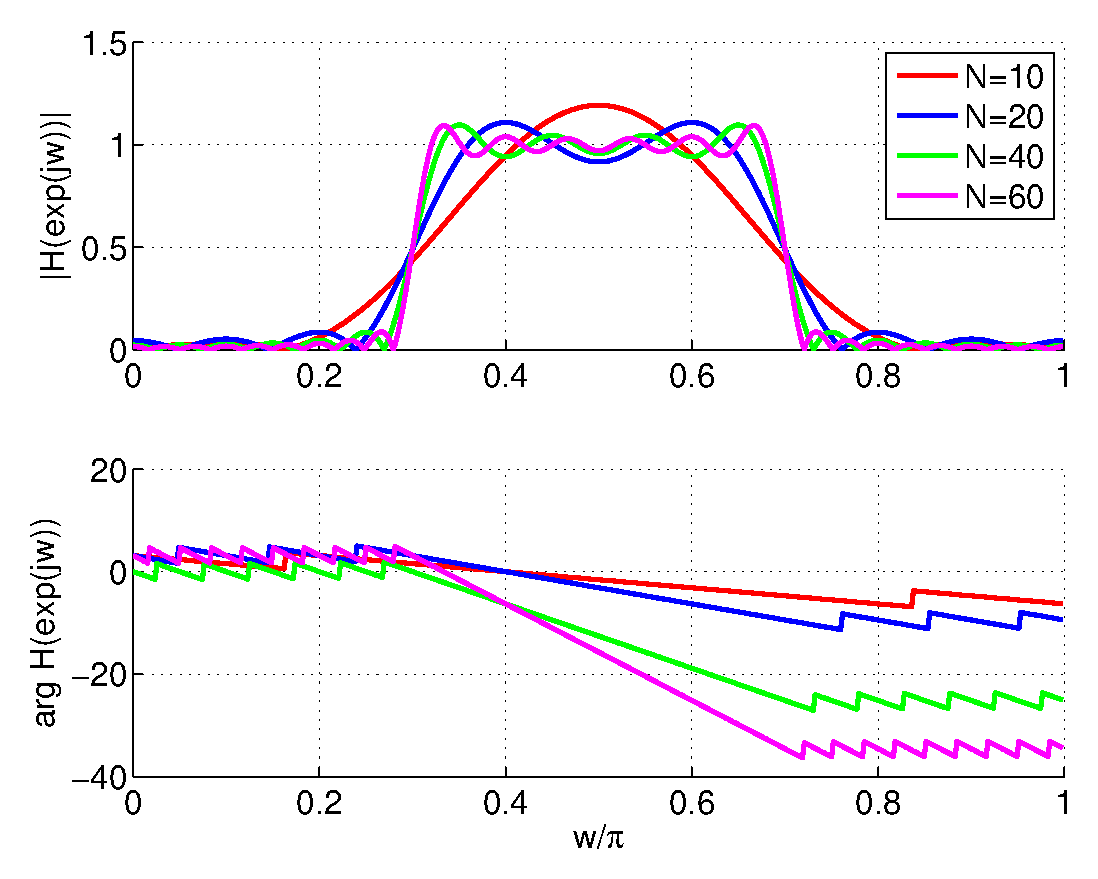
\includegraphics[width=4cm]{Figures/FIRPassTrunc.eps}
      
      Supresor de banda
      
      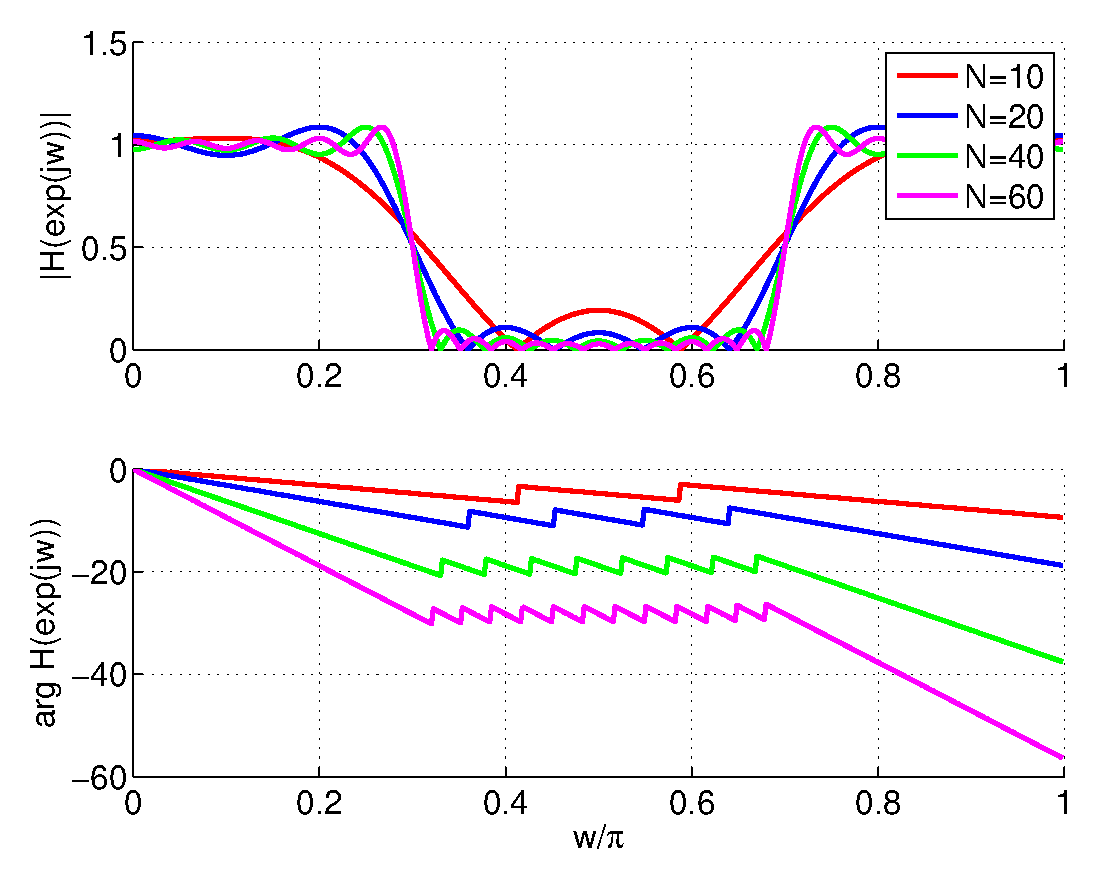
\includegraphics[width=4cm]{Figures/FIRStopTrunc.eps}
          
    \end{column}
  \end{columns}
  
  \scriptsize
  
  {
  
  Fase lineal ($-\omega N/2$, discont. $\pi$); tamaño rizos en el borde es constante; y según $N$ crece $\rightarrow \#_{rizos}$ crece, los rizos son más estrechos y la banda de transición decrece.
  }
  
\end{frame}
 
\begin{frame}
  \frametitle{Diseño del filtro FIR por truncamiento}
  \footnotesize
  \[\hspace{-1cm}\color{blue}h_w[n]\!=w[n]h_d[n] \Leftrightarrow H_w(\omega)=\frac{1}{2\pi}\int_{-\pi}^\pi H_d(\Omega)W(\omega-\Omega)d\Omega\]
  \vspace{-0.5cm}
  \hspace{0.3cm}\begin{columns}[c]
    \begin{column}{4.5cm}
      $N=2L+1$

      $w[n]=\left\{\begin{matrix*}[l]1 & |n|\leq L\\0 & |n|>L \end{matrix*}\right.$

      \vspace{0.1cm}
      $W(\omega)=\frac{\mathrm{sin}\left(\frac{\omega N}{2}\right)}{\mathrm{sin}(\frac{\omega}{2})}$
      
      \vspace{0.1cm}        
      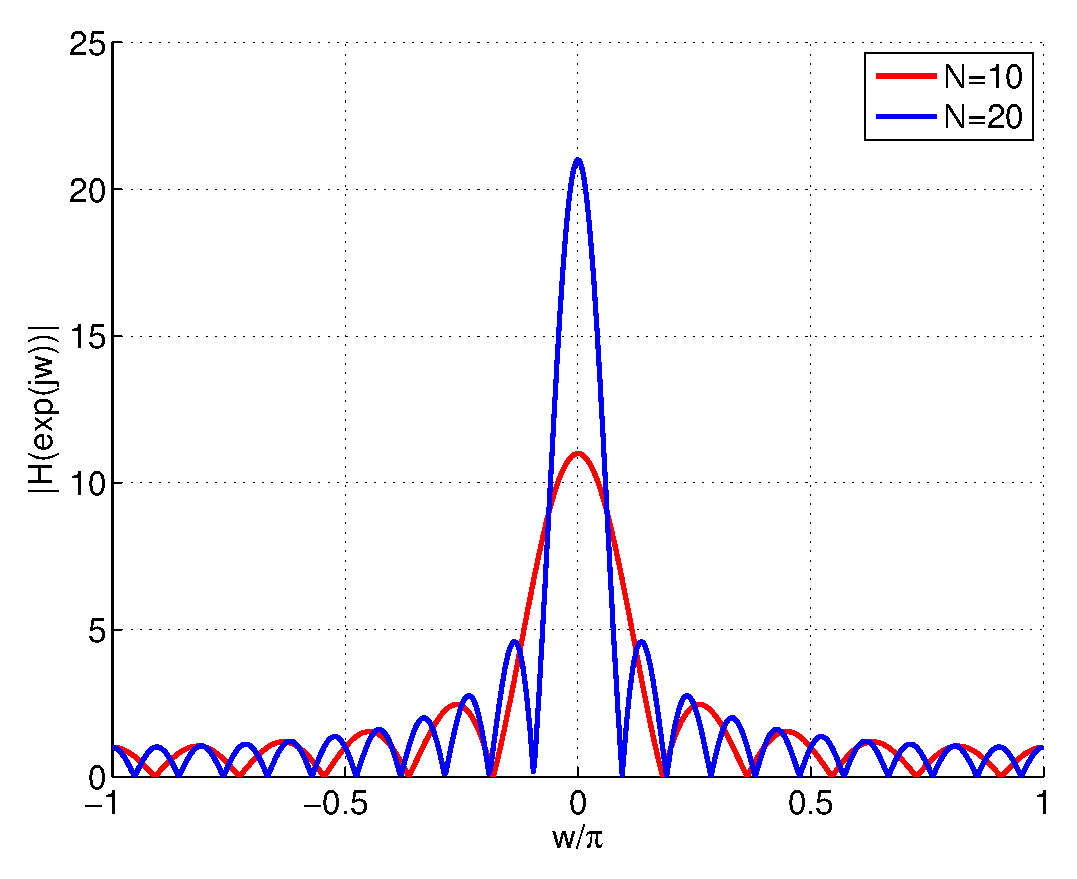
\includegraphics[width=3cm]{Figures/HwTrunc.eps}
    \end{column}
    \hspace{-2cm}\begin{column}{6.5cm}
      
      \vspace{0.1cm}
      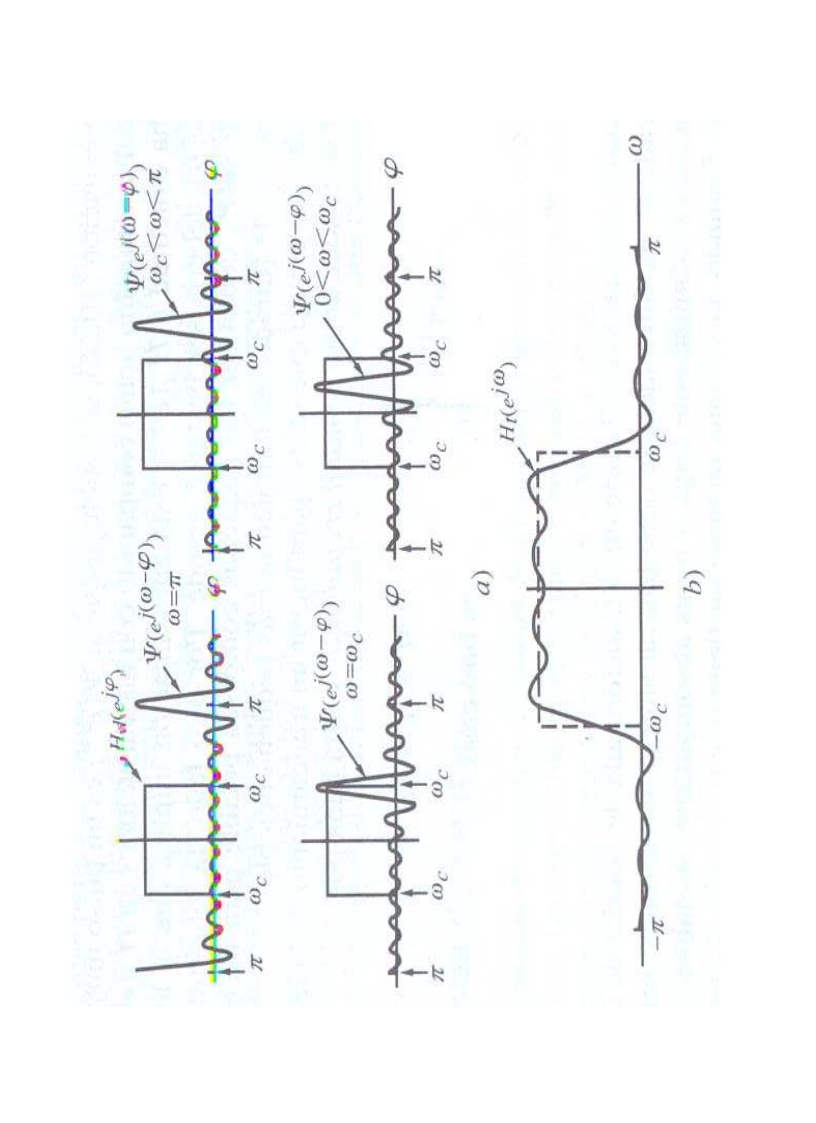
\includegraphics[trim=2cm 4cm 0cm 2cm, clip=true,angle=-90,width=6cm]{Figures/ConvTrunc}
    \end{column}
  \end{columns}
  \vspace{-0.4cm}
  \begin{alertblock}{Fenómeno de Gibbs}  
    La amplitud del rizado no depende de $N$. A medida que $N$ aumenta:    
    \begin{itemize}\scriptsize
      \item el lóbulo principal de $W(\omega)$ es más estrecho, pero su area no cambia.
      \item los rizos de $H_w(e^{j\omega})$ están más cerca de $\omega_c$ pero su tamaño no varía.
    \end{itemize}
  \end{alertblock}
\end{frame}

\begin{frame}{Órdenes Típicos en Aplicaciones de Audio}
  \begin{table}[]
      \centering
      \begin{tabular}{|c|c|}
          \hline
          \textbf{Aplicación} & \textbf{Orden Típico (N)} \\
          \hline
          Filtros básicos de audio & 50 - 200 \\
          Crossovers en sistemas de audio & 100 - 500 \\
          Cancelación de eco y reverberación & 500 - 2000 \\
          Procesamiento de alta calidad (Dolby, DAW) & 1000 - 5000 \\
          \hline
      \end{tabular}
      \begin{itemize}\footnotesize
          \item Filtros de orden alto ofrecen cortes más precisos pero introducen latencia.
          \item En tiempo real, se debe buscar un equilibrio entre precisión y eficiencia.
      \end{itemize}
  \end{table}
\end{frame}


\begin{frame}
  \frametitle{Diseño del filtro FIR con ventana fija}
  
  \vspace{-0.4cm}
  
  \footnotesize
  \begin{itemize}
    \item El fenómeno de Gibbs se debe a que $w[n]$ tiene una transición abrupta.
    \item Para mitigarlo, existen ventanas con transición mas suave ($-L\le n \le L$):
    \begin{itemize}
      \footnotesize
      \item Barlett: $w[n]=1-\frac{|n|}{L+1}$
      \item Hann: $w[n]=\frac{1}{2}\left [1+cos\left (\frac{2\pi n}{2L+1}\right )\right ]$
      \item Hamming: $w[n]=0.54+0.46 cos \left (\frac{2\pi n}{2L+1}\right )$
      \item Blackman: $w[n]=0.42+0.5 cos \left (\frac{2\pi n}{2L+1}\right )+0.08 cos \left (\frac{4\pi n}{2L+1}\right )$
    \end{itemize}
  \end{itemize}
  
  \vspace{0.2cm}
  \begin{columns}[c]
    \begin{column}{3cm}
      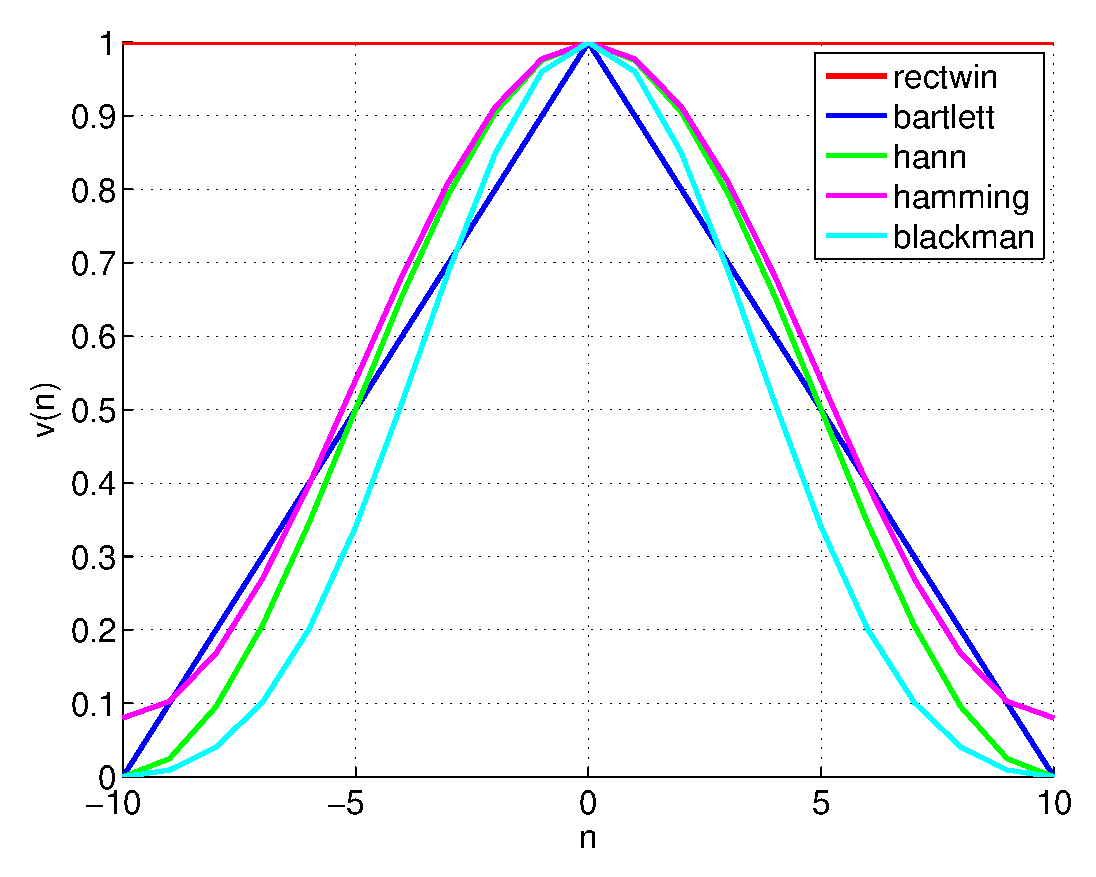
\includegraphics[trim=0cm 0cm 0cm 0cm, clip=true,angle=0,width=3.5cm]{Figures/hnWindow.eps}
    \end{column}
    \begin{column}{3cm}
      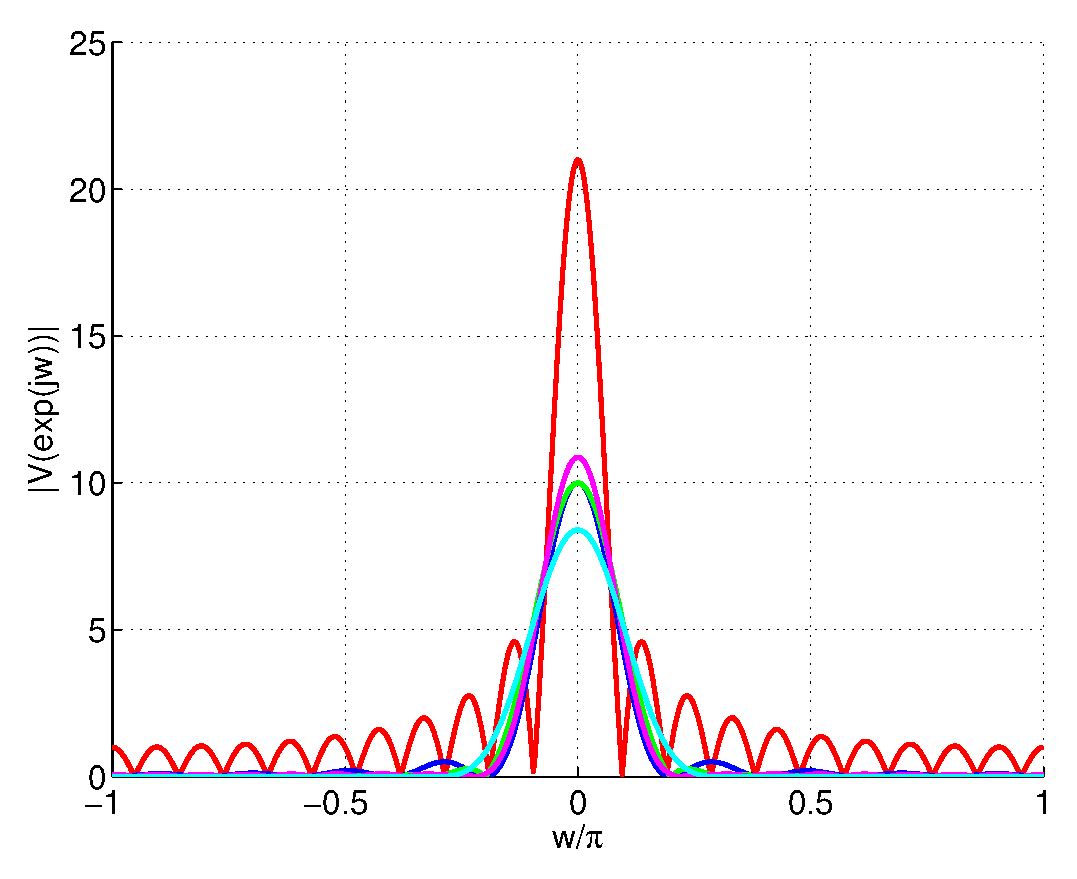
\includegraphics[trim=0cm 0cm 0cm 0cm, clip=true,angle=0,width=3.5cm]{Figures/HwWindow.eps}
    \end{column}
    \begin{column}{4.5cm}
      \scriptsize
      $\Delta_{ML}$: Ancho del lóbulo principal
      
      $A_{ML}$: Nivel relativo del l. p.

      \vspace{0.5cm}
      $\Delta_{ML},A_{ML}$ relacionados con $H_w(\omega)$
    \end{column}
  \end{columns}
  
\end{frame}


\begin{frame}
  \frametitle{Diseño del filtro FIR con ventana fija}
  
  \begin{columns}[c]
    \begin{column}{6.5cm}
      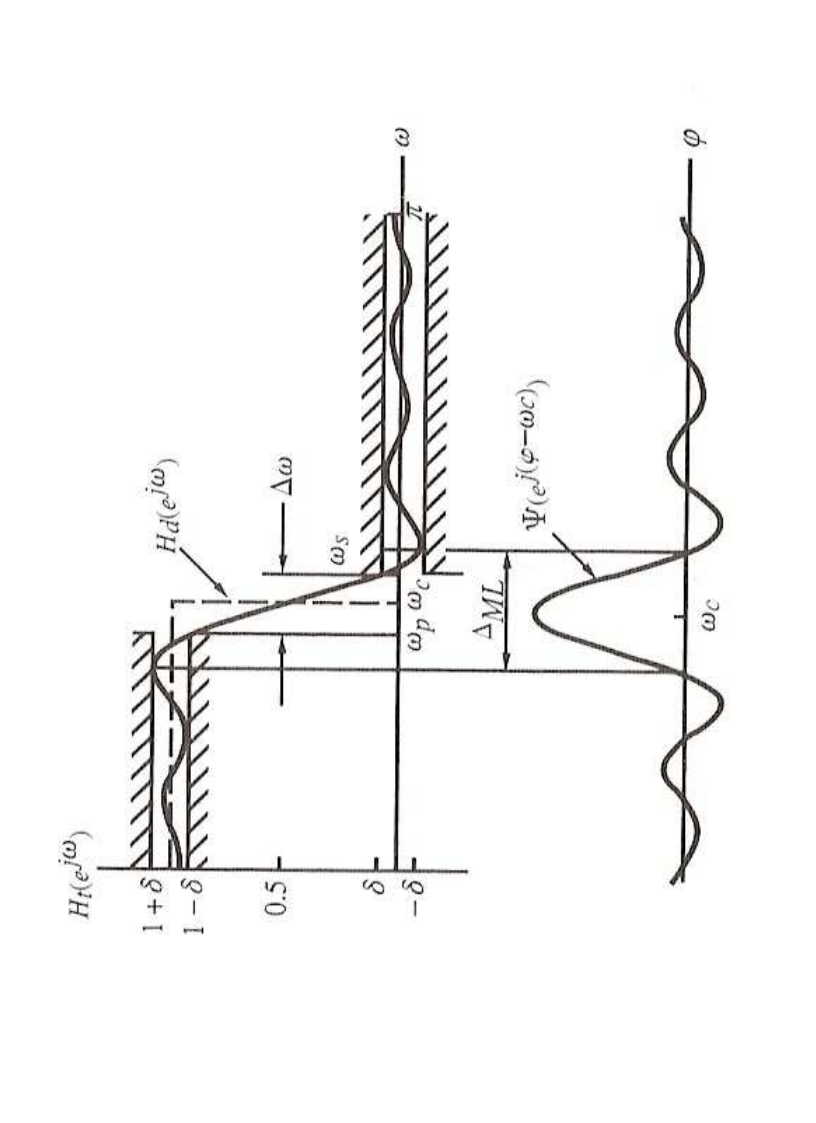
\includegraphics[trim=0cm 0cm 0cm 0cm, clip=true,angle=-90,width=7.5cm]{Figures/WindowFija1}
    \end{column}  
    \begin{column}{5.5cm}
      \begin{itemize}
        \footnotesize
        \item $|H(\omega_c)|=0.5$
        \item $\omega_c=\frac{\omega_p+\omega_s}{2}$
        \item $\Delta_\omega=\omega_s-\omega_p<\Delta_{ML}$
        \item Igual rizado $\delta$ en ambas bandas.
        \item Ventana fija $\Leftrightarrow$ rizado constante.
        \item $L$ aparece en la tabla como $M$.
      \end{itemize}
    \end{column}
  \end{columns}
  
  \vspace{-0.5cm}
  \visible<2->{
  \hspace{-0.3cm}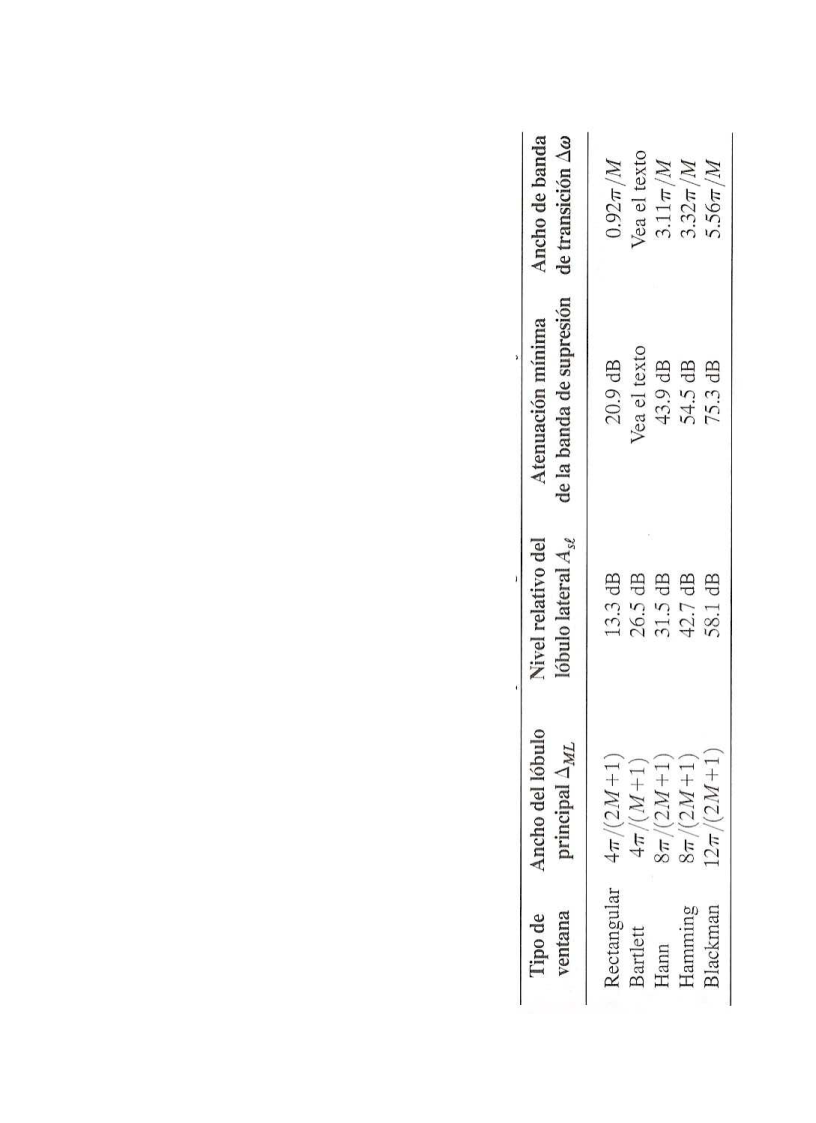
\includegraphics[trim=13cm 0cm 0cm 0cm, clip=true,angle=-90,width=12cm]{Figures/WindowFija2}}
  
\end{frame}
  
\begin{frame}
  \frametitle{Ejemplo FIR paso baja de ventana fija}
  
  \footnotesize
  
  \color{olivegreen}Diseñar un filtro paso bajo con las siguientes especificaciones:
  
  $\omega_p=0.3\pi$, $\omega_s=0.5\pi$, $\alpha_s=40dB$.  
  \color{gray}
  \vspace{-0.2cm}  
  \hspace{-0.3cm}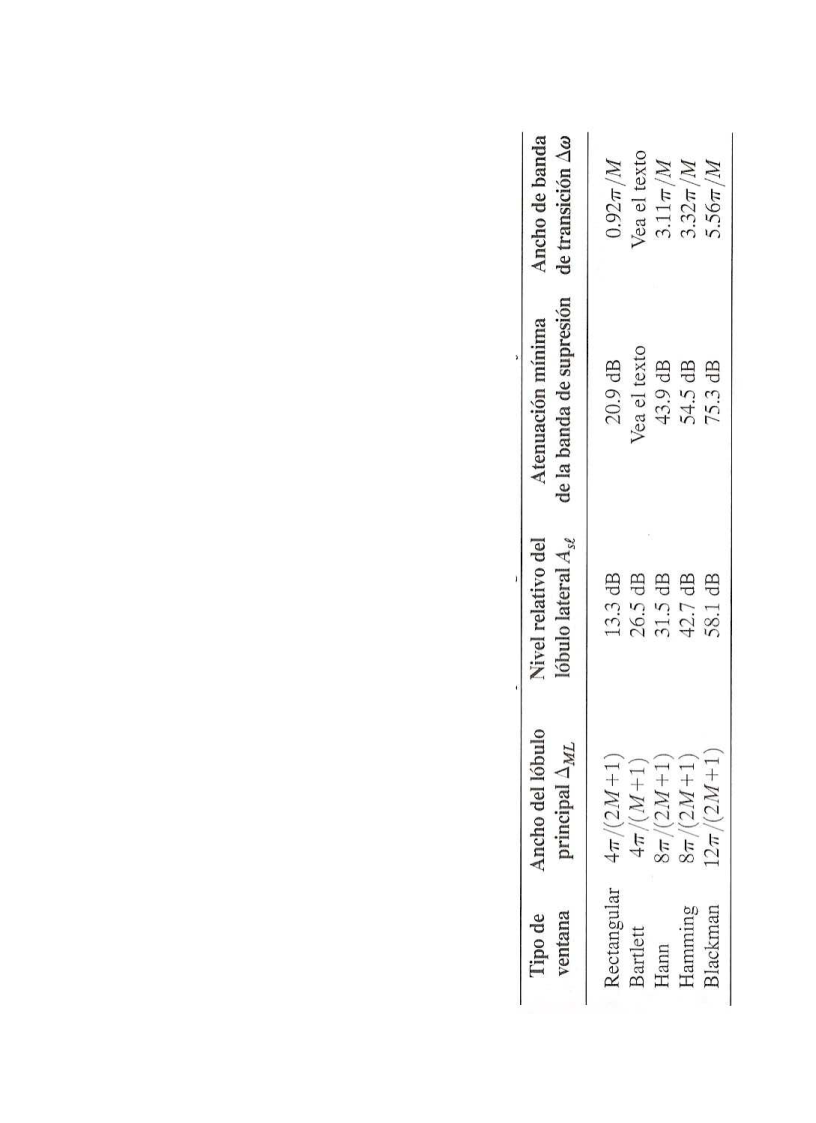
\includegraphics[trim=13.5cm 0cm 1cm 0cm, clip=true,angle=-90,width=10.5cm]{Figures/WindowFija2}
  
  \vspace{-0.2cm}
  \scriptsize
  $\omega_c= \frac{\omega_p+\omega_s}{2}=0.4\pi$   $\:\:\:\:\:\Delta_\omega=\omega_s-\omega_p=0.2\pi$
  
  \vspace{0.1cm}
  $\alpha_s=40dB$: Filtros posibles son Hann, Hamming, y Hamming\\
  Hann: $\Delta_\omega=3.11\pi/L  \rightarrow L=3.11\pi/\Delta_\omega=15.55 \rightarrow L=16$\\  
  Hamming: $\Delta_\omega=3.32\pi/L  \rightarrow L=3.32\pi/\Delta_\omega=16.6 \rightarrow L=17$\\  
  Blackman: $\Delta_\omega=5.56\pi/L  \rightarrow L=5.56\pi/\Delta_\omega=27.8 \rightarrow L=28$
  
  \vspace{-0.4cm}
  
  \begin{columns}[T]
    \hspace{1cm}\begin{column}{5.5cm}
      \lstinputlisting{./Matlab/FIREjemplo1.m}
    \end{column}
    \hspace{1cm}\begin{column}{4.5cm}
      \vspace{0.4cm}
      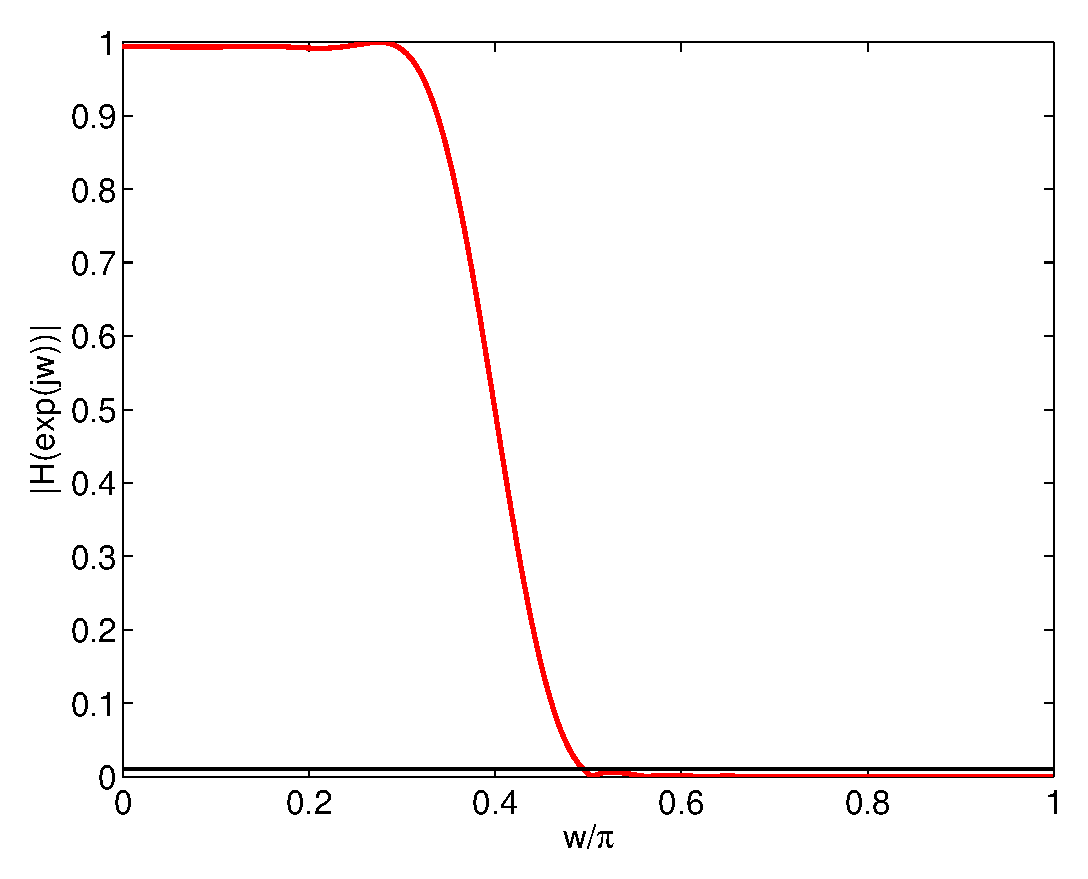
\includegraphics[trim=0cm 0cm 0cm 0cm, clip=true,angle=0,width=4cm]{Figures/FIREx1.eps}
    \end{column}
  \end{columns}
  
  \end{frame}
  
\begin{frame}
  \frametitle{Diseño del filtro FIR con ventana variable}
  \footnotesize
  \begin{itemize}
    \item Para tener control sobre el rizado, se pueden usar ventanas variables:
    \begin{itemize}
    \footnotesize
    \item \alert{Dolph-Chebyshev}: \texttt{ w=chebwin(2*L+1,Asl)}
    $w[n]=\frac{1}{2L+1}\left[ \frac{1}{\gamma}+\sum_{k=1}^L T_{2N}\left( \beta cos (\frac{k\pi}{2L+1})\right) cos (\frac{2nk\pi}{2L+1})\right]$
    
    $\gamma=\frac{\mathrm{amplitud \:\: lobulo  \:\: lateral}}{\mathrm{amplitud \:\: lobulo  \:\: principal}}$,  $\:\:\:\beta=cosh\left(\frac{1}{2L}acosh(1/\gamma)\right)$
    
    $T_l(x)=\left \{ \begin{array}{l}cos(l \cdot acos(x)), \:\: |x|<1\\cosh(l \cdot acosh(x)), \:\: |x|<1 \end{array}\right .$
    \alert{$\:\:2L=\frac{2.056\alpha_s-16.4}{2.285\Delta w}$}
    
    
    \vspace{0.2cm}
    
    
    \item \alert{Kaiser}: \texttt{ w=kaiser(2*L+1,beta)}
    
    \vspace{0.1cm}
    
    $w[n]=\frac{I_o\left(\beta \sqrt{1-(n/L)^2}\right)}{I_o\left(\beta\right)}$
    
    \vspace{0.1cm}
    
    $I_o(u)=1+\sum_{r=1}^\infty \left(\frac{(u/2)^r}{r!}\right).$
    
    $\beta=\left\{\begin{array}{l}0.11102(\alpha_s-8.7), \:\: \alpha_s>50\\0.5482(\alpha_s-21)^{0.4}+0.07886(\alpha_s-21), \:\: 50 \le \alpha_s \le 21\\0, c.c.\end{array} \right .$
    
    
    \alert{$2L=\frac{\alpha_s-8}{2.285\Delta w}$}
    
    \end{itemize}
  \end{itemize}
\end{frame}
  
\begin{frame}
  \frametitle{Ejemplo FIR paso bajo Dolph-Chebyshev}
  
  \footnotesize
  
  \color{olivegreen}Diseñar un filtro paso bajo con las siguientes especificaciones:
  
   $\omega_p=0.3\pi$, $\omega_s=0.5\pi$, $\alpha_s=40dB$.
  
  \color{gray}
  
   $\omega_c= \frac{\omega_p+\omega_s}{2}=0.4\pi$   $\:\:\:\:\:\Delta\omega=\omega_s-\omega_p=0.2\pi$
  
  $2L=\frac{2.056\alpha_s-16.4}{2.285\Delta\omega}  \rightarrow L=22.92  \rightarrow L=23$
  
  
  \begin{columns}[T]
    \hspace{1cm}\begin{column}{5.5cm}
      \lstinputlisting{./Matlab/FIREjemplo2.m}
    \end{column}
    \hspace{1cm}\begin{column}{4.5cm}  
      \vspace{0.4cm}
      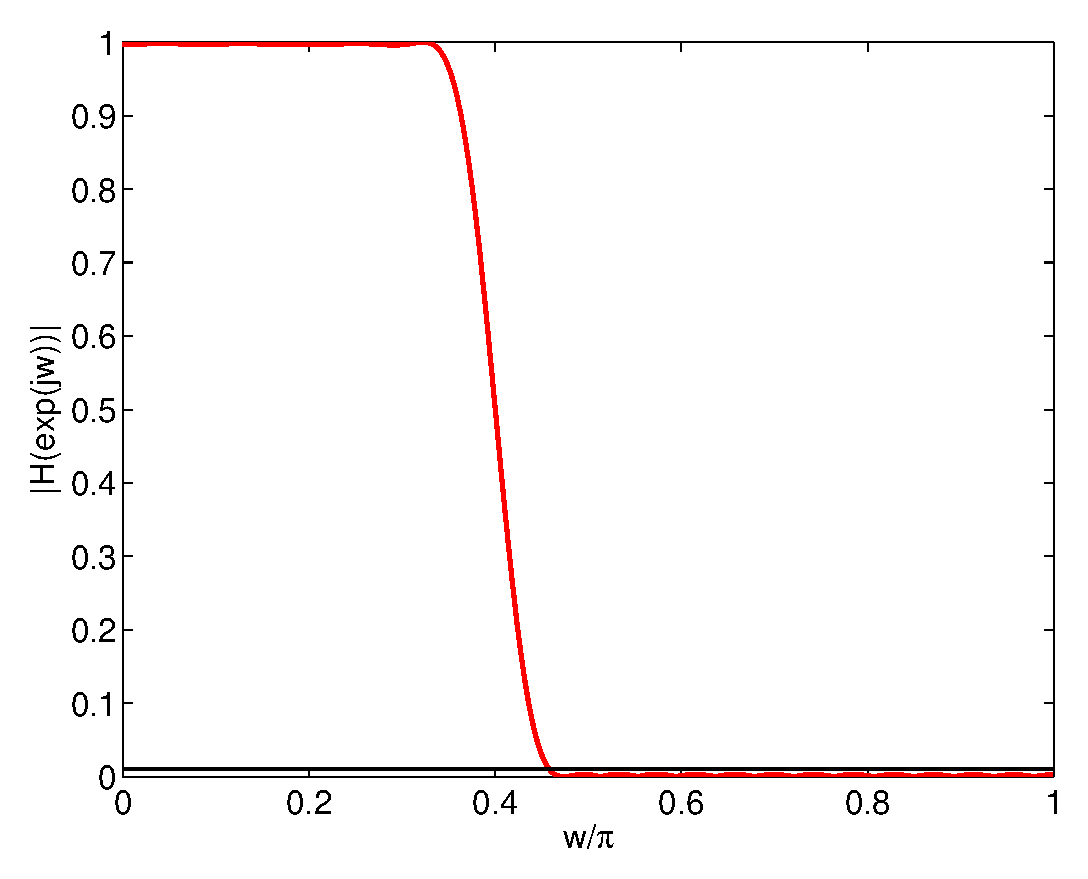
\includegraphics[trim=0cm 0cm 0cm 0cm, clip=true,angle=0,width=4.2cm]{Figures/FIREx2.eps}
    \end{column}
  \end{columns}  
\end{frame}
  
  
\begin{frame}
  \frametitle{Ejemplo FIR paso baja de ventana Kaiser}
  
  \footnotesize
  
  \color{olivegreen}Diseñar un filtro paso bajo con las siguientes especificaciones:
  
   $\omega_p=0.3\pi$, $\omega_s=0.5\pi$, $\alpha_s=40dB$.
  
  \color{gray}
  
   $\omega_c= \frac{\omega_p+\omega_s}{2}=0.4\pi$   $\:\:\:\:\:\Delta\omega=\omega_s-\omega_p=0.2\pi$
  
  $2L=\frac{\alpha_s-8}{2.285\Delta\omega}  \rightarrow L=11.14  \rightarrow L=12$
  
  $\beta=0.5482(\alpha_s-21)^{0.4}+0.07886(\alpha_s-21)=3.2784$
  
  \begin{columns}[T]
    \hspace{1cm}\begin{column}{5.5cm}
      \lstinputlisting{./Matlab/FIREjemplo3.m}
    \end{column}
    \hspace{1cm}\begin{column}{4.5cm}
      \vspace{0.4cm}
      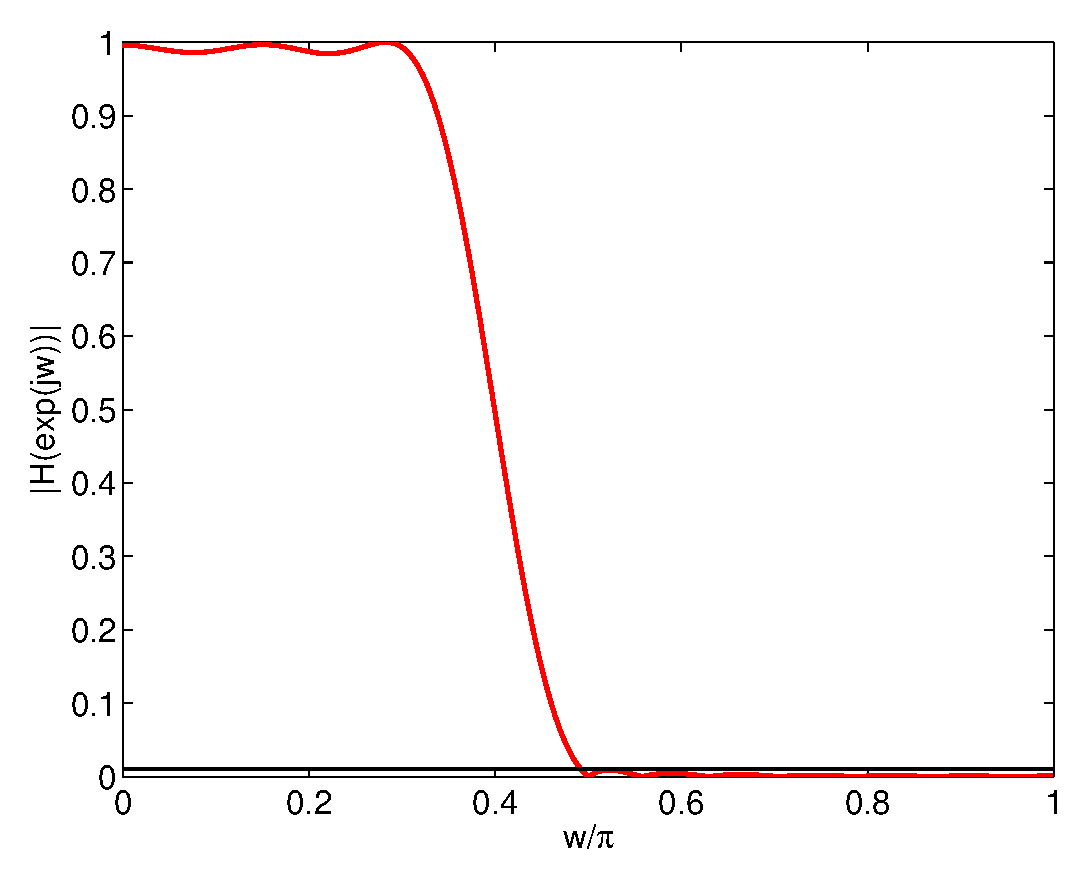
\includegraphics[trim=0cm 0cm 0cm 0cm, clip=true,angle=0,width=4.2cm]{Figures/FIREx3.eps}
    \end{column}
  \end{columns}
  
\end{frame}
  
  
\begin{frame}
  \frametitle{Diseño de filtros avanzados con Matlab}
  \footnotesize
  \begin{itemize}
    \item Matlab facilita los cálculos:
    \begin{itemize}
      \footnotesize
      \item Ordenes relacionadas con la ventana de Kaiser:
      \texttt{[N,wc,beta,type]=kaiserord([wp,ws],[A1,A2],[dp,ds])}\\      
      \texttt{window=kaiser(N+1,beta);}\\      
      \texttt{h=fir1(N,wc,type,window);}
      
      \item Ordenes para el diseño de filtros  multinivel:
      \texttt{ws=[w0,w1,...,wM];}\\
      \texttt{A=[A0,A1,...AM];}\\
      \texttt{h=fir2(N,ws,A,window)};
    \end{itemize}
  \end{itemize}
\end{frame}

\begin{frame}
  \frametitle{Ejemplo FIR paso alto de ventana Kaiser}  
  \footnotesize
  \color{olivegreen}Diseñar un filtro paso alto con las siguientes especificaciones:\\
  $\omega_p=0.55\pi$, $\omega_s=0.4\pi$, $\delta_s=0.01$.
  
  \color{gray}
  
  \begin{columns}[T]
    \begin{column}{6.5cm}
      \lstinputlisting{./Matlab/FIREjemplo4.m}
    \end{column}
    \hspace{-0.5cm}\begin{column}{4.5cm}
      \vspace{0.4cm}
      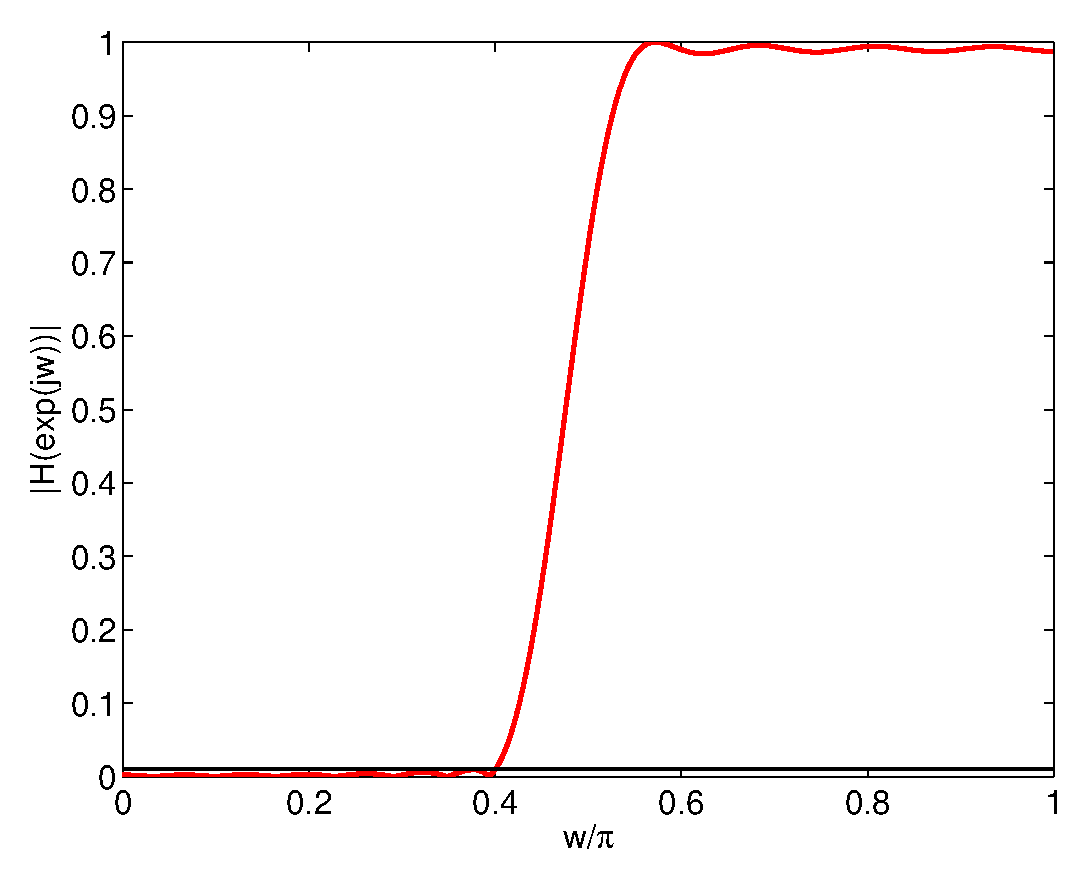
\includegraphics[trim=0cm 0cm 0cm 0cm, clip=true,angle=0,width=4.2cm]{Figures/FIREx4.eps}
    \end{column}
  \end{columns}
  
\end{frame}

\begin{frame}
  \frametitle{Ejemplo FIR multibanda}  
  \footnotesize  
  \color{olivegreen}Diseñar un filtro multibanda con ventana de Hamming con las siguientes especificaciones:
  
  w=[0,0.28,0.3,0.5,0.52,1];
  
  A=[0.3,0.3,1.0,1.0,0.7,0.7];
  
  \color{gray}
  
  \begin{columns}[T]
    \begin{column}{6.5cm}
      \lstinputlisting{./Matlab/FIREjemplo5.m}
    \end{column}
    \hspace{-0.5cm}\begin{column}{4.5cm}
      \vspace{0.4cm}
      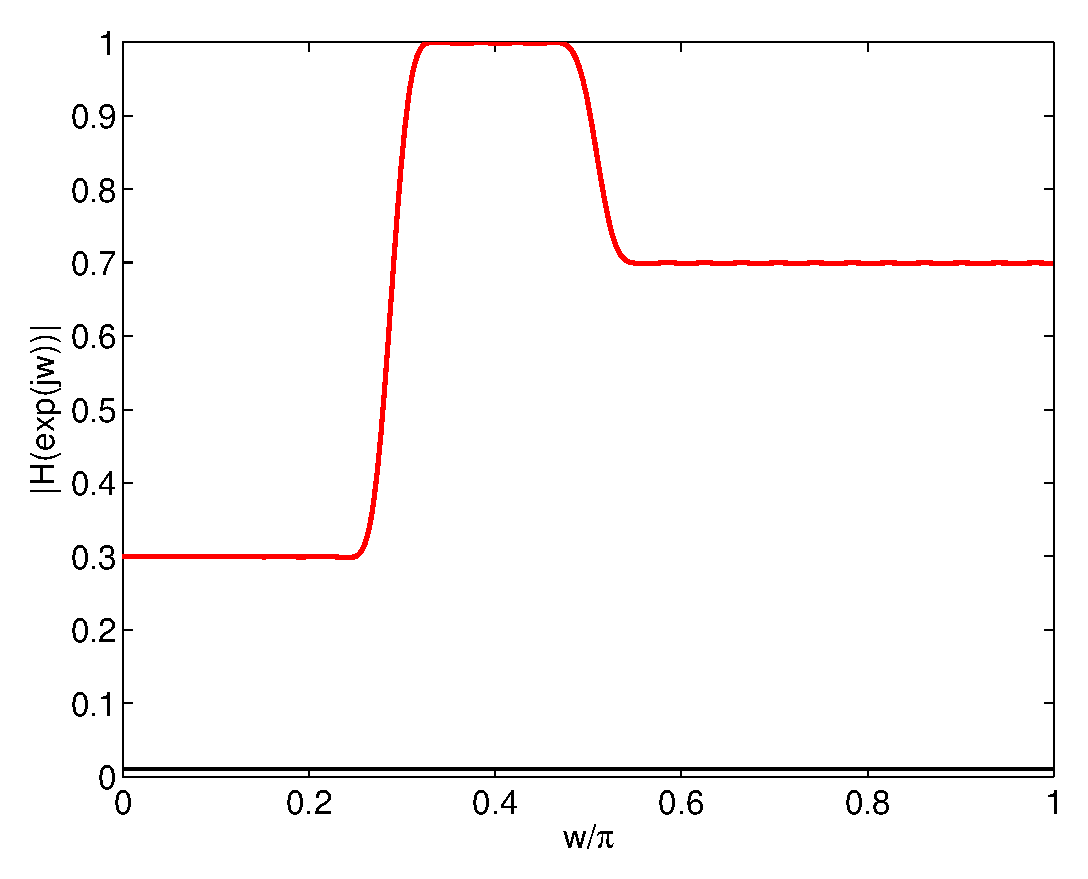
\includegraphics[trim=0cm 0cm 0cm 0cm, clip=true,angle=0,width=4.2cm]{Figures/FIREx5.eps}  
    \end{column}
  \end{columns}
\end{frame}

\begin{frame}
  \frametitle{Conceptos importantes}

  \begin{itemize}
    \item \alert{Diseño FIR por truncamiento y retardo}
    \begin{itemize}
      \item Truncamiento a $N=2L+1$ muestras.
      \item Retardo de $L$ muestras para hacer causal.
    \end{itemize}
    \item \alert{Ventana fija}
    \begin{itemize}
      \item \textbf{Fenómeno de Gibbs}: rizado no varía con $N$.
      \item El rizado solo depende de la ventana:\\\emph{rectangular, Hamming, Barlett, Hanning, etc}.
    \end{itemize}
    \item \alert{Ventana variable}
    \begin{itemize}
      \item La ventana es ajustable (\emph{Dolph-Chebishev, Kaiser}).
      \item El rizado se puede controlar.
    \end{itemize}
  \end{itemize}
\end{frame}


\end{document}
